\begin{figure}[htbp]
\centering
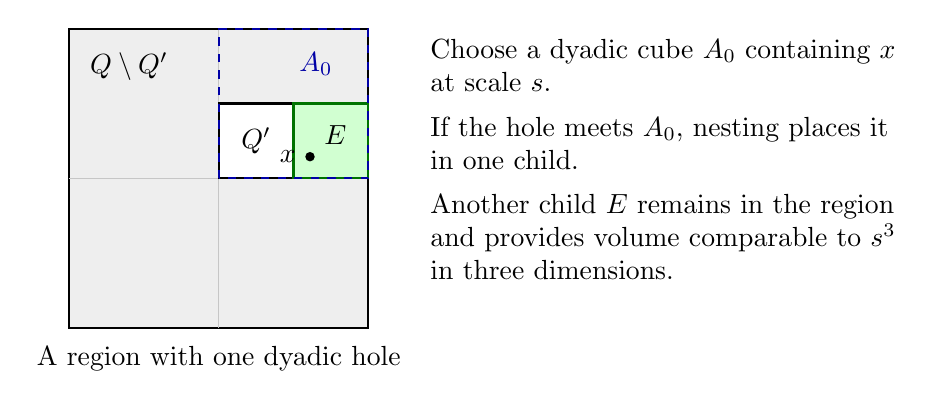
\begin{tikzpicture}[scale=0.95]
 \fill[gray!13] (0,0) rectangle (4,4);
 \draw[thick] (0,0) rectangle (4,4);
 \draw[gray!45] (2,0)--(2,4) (0,2)--(4,2);
 \fill[white] (2,2) rectangle (3,3);
 \draw[thick] (2,2) rectangle (3,3);
 \fill[green!18] (3,2) rectangle (4,3);
 \draw[green!45!black,thick] (3,2) rectangle (4,3);
 \draw[blue!65!black,dashed,thick] (2,2) rectangle (4,4);
 \fill (3.22,2.29) circle (1.8pt);
 \node[anchor=east] at (3.16,2.29) {$x$};
 \node at (2.5,2.5) {$Q'$};
 \node at (3.56,2.58) {$E$};
 \node[blue!65!black] at (3.3,3.53) {$A_0$};
 \node at (0.8,3.5) {$Q\setminus Q'$};
 \node[anchor=north] at (2,-0.12) {A region with one dyadic hole};
 \node[align=left,anchor=west,text width=6.0cm] at (4.7,2.25)
 {Choose a dyadic cube $A_0$ containing $x$ at scale $s$.\\[4pt]
  If the hole meets $A_0$, nesting places it in one child.\\[4pt]
  Another child $E$ remains in the region and provides volume
  comparable to $s^3$ in three dimensions.};
\end{tikzpicture}
\caption{A two-dimensional illustration of the thickness argument in
Lemma~\ref{mot:partition}.  The volume estimate is proved for
three-dimensional cubes.  It holds near the hole as well as near the
outer boundary, and survives every rigid motion.  This makes the
packing argument independent of the depth of the dyadic subdivision.}
\label{mot:partition-figure}
\end{figure}
